
\chapter{Конструкторская часть}\label{Konstruct}
%\addcontentsline{toc}{chapter}{2 Конструкторская часть}

\section{Схемы алгоритмов}\label{SchemaAlg}


\subsection{Схема стандартного алгоритма умножения матриц}\label{SchemaMatrixMultiply}

На рисунке \ref{ris:schemastandart} показана схема алгоритма расчета расстояния Левенштейна матричным способом.

\begin{figure}[H]
  \center{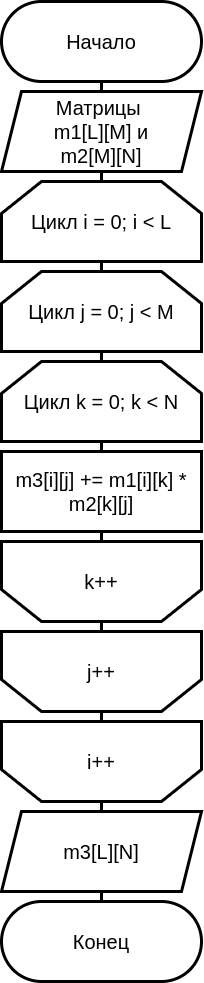
\includegraphics[scale=0.35]{l1.schemastandart}}
  \caption{Схема стандартного алгоритма умножения матриц}
  \label{ris:schemastandart}
\end{figure}


\subsection{Схема алгоритма Винограда}\label{SchemaMatrixVinograd}

На рисунке \ref{ris:schemavinograd} показана схема алгоритма расчета расстояния Левенштейна с помощью рекурсии.

\begin{figure}[H]
    \center{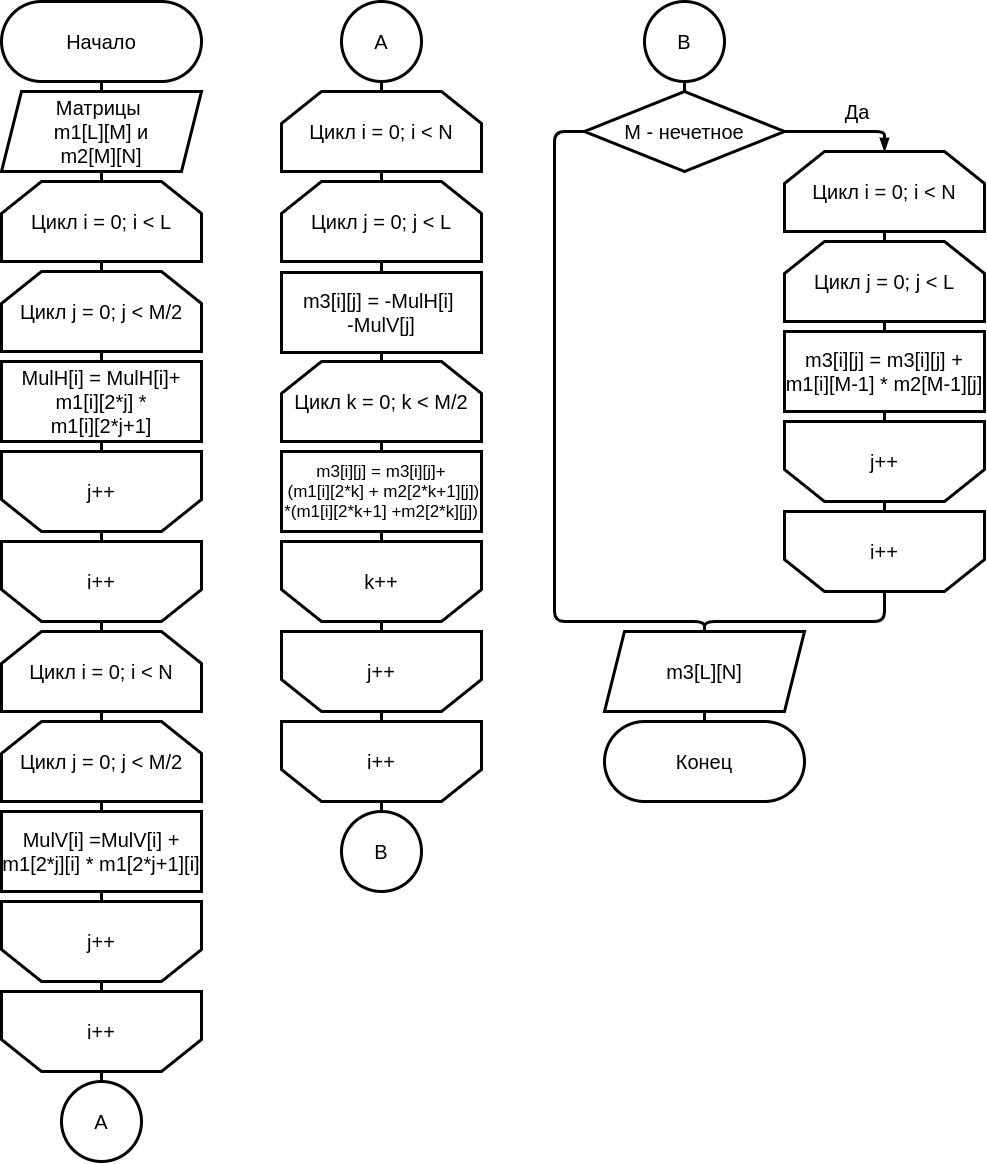
\includegraphics[scale=0.35]{l1.schemavinograd}}
    \caption{Схема алгоритма Винограда}
    \label{ris:schemavinograd}
\end{figure}

\subsection{Схема оптимизированного алгоритма Винограда}\label{SchemaMatrixOptimVinograd}

На рисунке \ref{ris:schemaoptvinograd} показана схема алгоритма расчета расстояния Левенштейна с помощью рекурсии.

\begin{figure}[H]
    \center{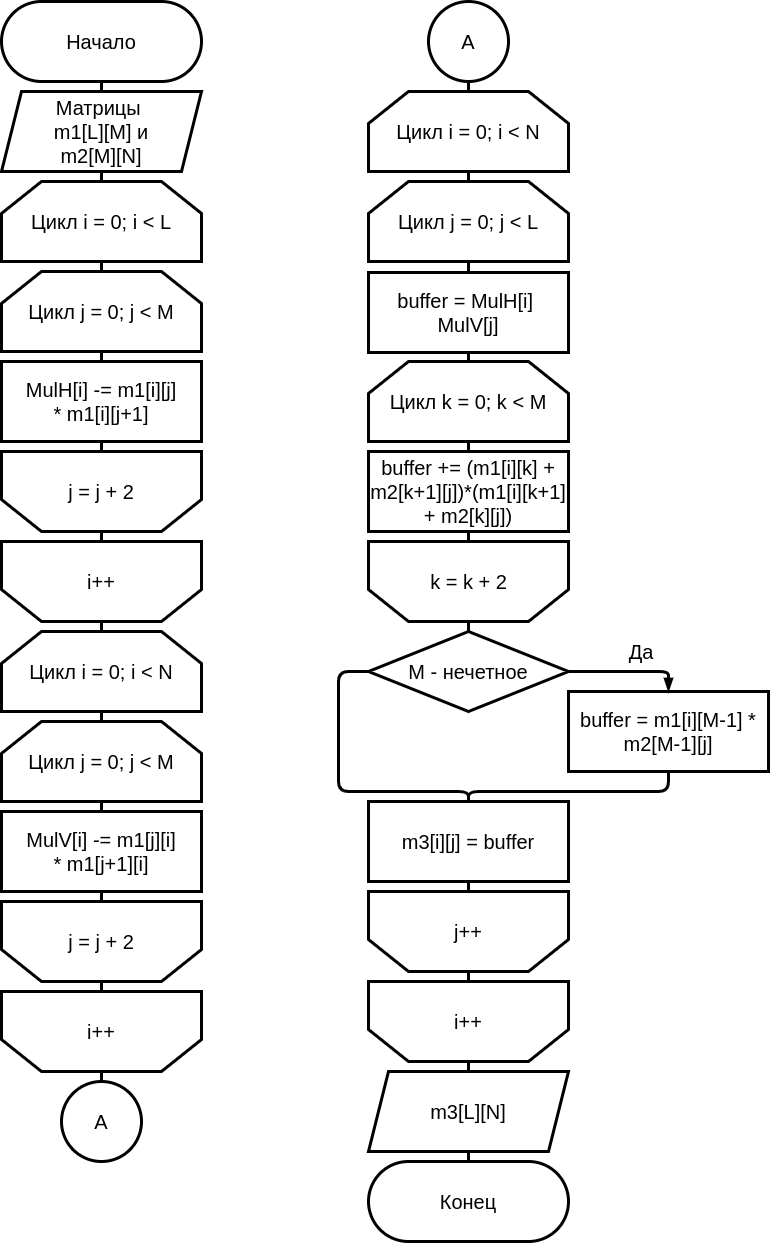
\includegraphics[scale=0.35]{l1.schemaoptvinograd.png}}
    \caption{Схема оптимизированного алгоритма Винограда}
    \label{ris:schemaoptvinograd}
\end{figure}

\section{Трудоемкость алгоритмов}\label{Complecity}

\subsection{Трудоемкость стандартного алгоритма умножения матриц}\label{ComplecityMatrixMultiply}

$ f = 2 + L \cdot (2 + 2 + M \cdot (2 + 2 + N \cdot (2 + 8 + 1 + 1 + 2)))$\label{formula:resmulmat}

\subsection{Трудоемкость алгоритма Винограда}\label{ComplecityMatrixVinograd}

Для наглядного подсчета можно заполнить таблицу \ref{tab:matrixComplexityVinograd}, а после посчитать общую трудоемкоть.

\begin{table}[ht]
    \caption{Трудоемкость алгоритма Винограда}
\begin{tabular}{| l | l |}\hline
    Часть алгоритма & Трудоемкость \\ \hline
    Инициализация MulH и MulV & 2\\ \hline
    Заполнение MulH & $2 + L \cdot (2 + 2 + M/2 \cdot (3 + 6 + 6))$\\ \hline
    Заполнение MulV & $2 + N \cdot (2 + 2 + M/2 \cdot (3 + 6 + 6))$\\ \hline
    Подсчет результата & $2 + L \cdot (2 + 2 + N \cdot (2 + 7 + 2 + M/2 \cdot (3 + 23)))$\\ \hline
    Усл. оператор (на нечет. m) & $2 $\\ \hline
    Тело усл. оператора (нечет. m)& $2 + N \cdot (2 + 2 + L\cdot(9+2))$\\ \hline

\end{tabular}
\label{tab:matrixComplexityVinograd}
\end{table}

Общая трудоемкость:

$
f = 2 + 2 + L \cdot (2 + 2 + M/2 \cdot (3 + 6 + 6)) + 2 + N \cdot (2 + 2 + M/2 \cdot (3 + 6 + 6)) + 2 + 
L \cdot (2 + 2 + N \cdot (2 + 7 + 2 + M/2 \cdot (3 + 23))) + 2 + 
\left\{
    \begin{array}{ccc}
        2 + N \cdot (2 + 2 + L\cdot(13+2)), (m-\text{нечет.})\\
        0, (m-\text{чет.}) 
    \end{array}
\right\}
$ \label{formula:bigresalgvinograd}

$
f = 13 \cdot M \cdot N \cdot L + 11\cdot L \cdot N + 7,5\cdot M \cdot N + 7,5\cdot M \cdot L + 8 \cdot L + 4 \cdot N + 10 +
\left\{
    \begin{array}{ccc}
        15\cdot N\cdot L + 4\cdot N + 2, (m-\text{нечет.})\\
        0, (m-\text{чет.}) 
    \end{array}
\right\}
$ \label{formula:smallresalgvinograd}

\subsection{Трудоемкость оптимизированного алгоритма Винограда}\label{ComplecityMatrixOptimVinograd}

Таблица трудоемкостей частей алгоритма: \ref{tab:matrixComplexityOptVinograd}, а после посчитать общую трудоемкоть.

\begin{table}[ht]
    \caption{Трудоемкость оптимизированного алгоритма Винограда}
\begin{tabular}{| l | l |}\hline
    Часть алгоритма & Трудоемкость \\ \hline
    Инициализация MulH и MulV & 2\\ \hline
    Заполнение MulH & $2 + L \cdot (2 + 2 + M/2 \cdot (2 + 8))$\\ \hline
    Заполнение MulV & $2 + N \cdot (2 + 2 + M/2 \cdot (2 + 8))$\\ \hline
    Подсчет результата & $2 + L \cdot (2 + 2 + N \cdot (2 + 10 + M/2 \cdot (2 + 14)))$\\ \hline
    Усл. оператор (на нечет. m) & $2 \cdot N \cdot L$\\ \hline
    Тело усл. оператора (нечет. m)& $9\cdot N\cdot L$\\ \hline

\end{tabular}
\label{tab:matrixComplexityOptVinograd}
\end{table}

Общая трудоемкость:

$
f = 2 + 2 + L \cdot (2 + 2 + M/2 \cdot (2 + 8)) + 2 + N \cdot (2 + 2 + M/2 \cdot (2 + 8)) + 2 + 
L \cdot (2 + 2 + N \cdot (2 + 10 + M/2 \cdot (2 + 14))) + 2 \cdot N \cdot L + 
\left\{
    \begin{array}{ccc}
        9\cdot N\cdot L, (m-\text{нечет.})\\
        0, (m-\text{чет.}) 
    \end{array}
\right\}
$ \label{formula:bigresoptalgvinograd}

$
f = 8 \cdot M \cdot N \cdot L + 14\cdot L \cdot N + 5\cdot M \cdot N + 5\cdot M \cdot L + 8 \cdot L + 4 \cdot N + 8 +
\left\{
    \begin{array}{ccc}
        9\cdot N\cdot L, (m-\text{нечет.})\\
        0, (m-\text{чет.}) 
    \end{array}
\right\}
$ \label{formula:smallresoptalgvinograd}

\section{Сравнительный анализ трудоемкостей алгоритмов}\label{Konstructanalis}

Сравнив трудоемкости, можно сделать вывод, что самым быстрым алгоритмом из рассматриваемых является оптимизированный алгоритм Винограда. 
По трудоемкости он быстрее обычного алгоритма Винограда, значит он был оптимизирован верно (проделанные над ним изменения можно называть оптимизацией). Самым неэффективным по времени
алгоритмом является стандартный алгоритм умножения матриц. Проверим предположения, проанализировав полученные экспериментально данные.

\section{Структуры данных}\label{Structs}

При реализации приведенных алгоритмов потребуются следующие типы данных: матрица, массив.

\section{Тестирование}\label{Testing}

\subsection{Классы эквивалентности}\label{TestingClasses}

Для алгоритма умножения матриц можно выделить следующие классы эквивалентности (даны матрицы N*M и K*S):

\begin{enumerate}
    \item $M \neq K $
    \item $M = K $
\end{enumerate}

\subsection{Способы тестирования}\label{TestingMethods}

При разработке программы удобно использовать следующие методы тестирования:

\begin{enumerate}
    \item Модульные тесты 
    \item Функциональные тесты 
\end{enumerate} 

\section{Вывод конструкторской части}\label{KonstructResult}
На основе данных, полученных в аналитическом разделе, были построены схемы используемых алгоритмов,
выделены необходимые для реализации структуры данных и методы тестирования.

